\section{Experiments and Evaluation}\label{sec:experiments}
% Describe our results based on different number of producer and consumer numbers. 
We have implemented and evaluated our event processing architecture in Python and Java. We have run multiple experiments  to be 
able to select the right stream processing architecture for this task. Our experiments include a set of experiments with varying 
numbers of event producers and consumers threads, as well as other experiments with different number of threads and queue buffer sizes. 

The main computation for query 1 and query 2 is a very small computation to get the last prices from a dictionary of stock symbols and then 
check the two values of EMA 38 and 38 to find out the breakouts. We have profiled our implement and confirmed that the main implemented system 
is an I/O bounded application rather than a CPU bounded application because of a quick computation for query 1 and 2. The main time was 
invested to get the data from the network (which we improved by having multiple producers), and then organizing the stock price 
dictionaries and iterating over the single events in an event batch. 

By using vectorized bulk operations we can avoid the linear time of iterations over the batch of events. This is implemented by using 
vectorization within each of our multi-threaded consumers. 

% Experiments with different number of event producer threads and consumer threads. 
We have experimented with different number of producers and consumers. 
Figure \ref{} depicts query 2 throughput results for different number of producers and consumers. 
This results are produced by using the benchmark system provided by the DEBS 2022 grand challenge. 


\begin{figure}[]
    \begin{center}
        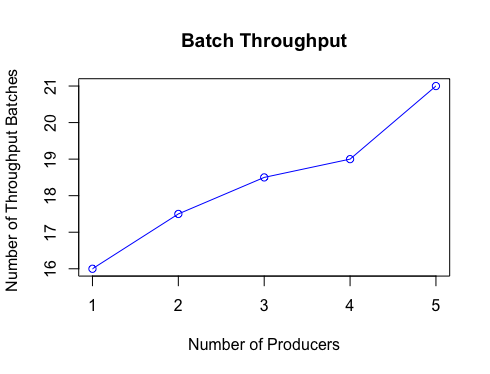
\includegraphics[width=0.5\textwidth]{./images/throughput.png}
        \caption{Query 2 throughput for different number of Producers. (Batch Size 1k)}
        \label{fig:evaluation}
    \end{center}
\end{figure}


%TODO!: Experiment with different architectures if we have any. 
